
%----------------------------------------------------------------------------------------
%	Lecture 8
%----------------------------------------------------------------------------------------

\chapter{Curve Sketching}

\bigbreak

{\bf Goal: } To draw the graph of $f$ using behaviour of $f'$ and $f''$.
We want to graph qualitatively but not to scale.


\section{Rules for Curve Sketching}

\begin{enumerate}
	\item Plot the discontinuities of $f$ especially the infinite ones.
	\item Find the critical points. These are points where $f'(x) = 0$.
	\item Plot the critical points and critical values. Decide the sign of $f'(x)$ in between critical points.
	\item Find and plot the zeros of $f$. Only do this if its relatively easy.
	\item Determine the behaviour at end points (or at $x = \pm \infty$)
\end{enumerate}


\section{Second Derivative Information}

When $f'' > 0, f'$ is increasing. When $f'' < 0, f'$ is decreasing.


\begin{figure}[ht!]
	\centering
	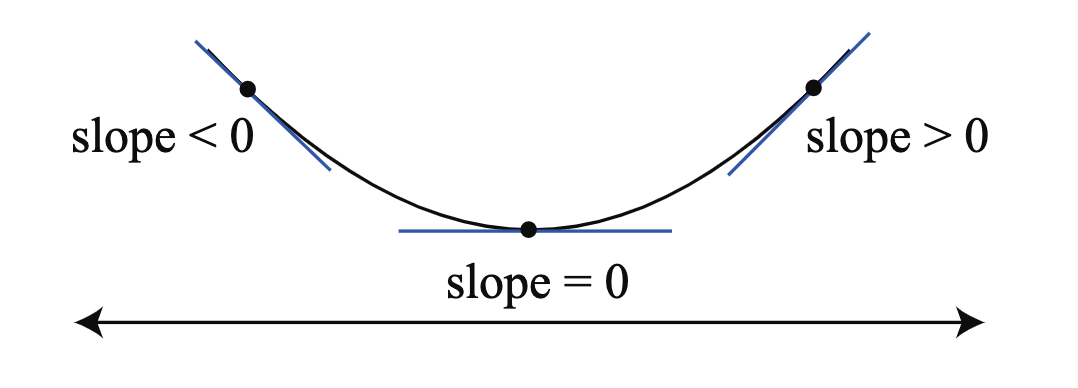
\includegraphics[scale=0.65]{./images/lecture_8_figure_1.png}
	\caption{$f$ is convex (concave up). The slope increases from negative to positive as $x$ increases.}
\end{figure}


\begin{figure}[ht!]
	\centering
	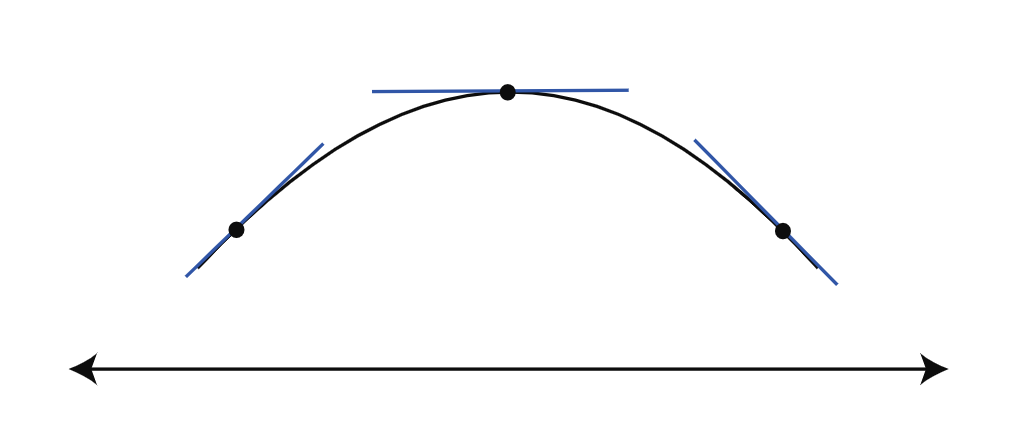
\includegraphics[scale=0.65]{./images/lecture_8_figure_2.png}
	\caption{$f$ is concave down. The slope decreases from positive to negative as $x$ increases.}
\end{figure}


Therefore, the sign of the second derivative tells us about the concavity/convexity of the graph.
Thus the second derivative is good for two purposes.

\begin{enumerate}
	\item Deciding whether a critical point is minimum or maximum. This is known as the \underline{second derivative} test.
	\begin{center}
	\begin{tabular}{ |c|c|c| }
		\hline
		$f'(x)$ & $f''(x)$ & Critical point is a: \\
		\hline
		$0$ & negative & maximum \\
		\hline
		$0$ & positive & minimum \\
		\hline
	\end{tabular}
	\end{center}
	\item Concave/Convex ``decoration.''
\end{enumerate}

The points where $f'' = 0$ are called \textit{inflection points}.
Usually these are the points where graph changes from concave up to concave down, or vice-versa.

\begin{figure}[ht!]
	\centering
	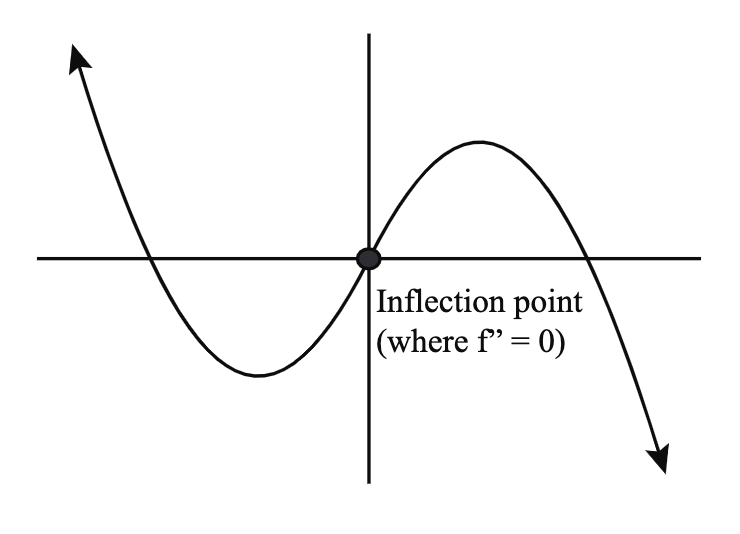
\includegraphics[scale=0.65]{./images/lecture_8_figure_3.png}
	\caption{Inflection point: $y = 3x - x^3, y'' = -6x = 0$, at $x = 0$.}
\end{figure}